
%%%%%%%%%%%%%%%%% Introduction to the Assignment %%%

In this Assignment, \textit{\textbf{Problem 5 - Optimization of phased array antenna radiation pattern and array configuration}}, a phased array consisting of 64 lined up isotropic antennas shall be configured and its configuration investigated. The antenna beam shall be a composite vertical beam in vertical direction, with a operating frequency of 53 MHz.

The design shall be done according to the given equation \ref{eq:orig} in Röttger, chap. 2.1 \citep{roettger1989instrumental}.

\begin{equation}
	E(\delta) = \sum_{n=1}^N E_n(\delta) \exp \Bigg(i\Big(\sin(\delta)\frac{2 \pi (n-1)d}{\lambda}  + \varphi_n \Big)\Bigg)
	\label{eq:orig}
\end{equation}

Additionally, the variables of the design shall be investigated and proper values found.

%%%%%%%%%%%%%%%%% TASK intro %%%
\section{Array Factor Derivation}
\label{chap:derivation}
To understand the different implications of the variables of the given equation \ref{eq:orig}, it is helpful to derive the equation. Also one should take into account the pattern multiplication theorem \citep{donohoe:lecture}, where the array pattern is given as product of each array element pattern times the array factor (AF).
Based on the given boundary condition to use an isotropic radiator (located at origin), the initial equation to start with is the one for the (far) field of an isotropic radiator

\begin{equation}
	E = I_0 \frac{e^{-jkr}}{4\pi r}
	\label{eq:iso_radiator}
\end{equation}
with $I_0$ as current on the antenna, $k$ as wavenumber given by $k = \frac{2\pi}{\lambda}$ and $r$ the distance to the target.
Assuming that the current magnitudes of the array elements are equal, and using the first (origin) array element as phase reference, means this array element has $\varphi = 0$ \citep{donohoe:lecture}, the currents on the array elements are as follows:

\begin{equation}
	I_1 = I_0 , \quad I_2 = I_0 \exp(j \varphi_{2}), \quad \dots \quad I_N = I_o \exp(j \varphi_{N})
	\label{eq:currents}
\end{equation}
with $N$ being the number of array elements.

The distance to the target for each array element can be easily derived using simple geometry (c.f. fig. \ref{fig:radiationPattern}).

\begin{figure}[!h]
\centering
	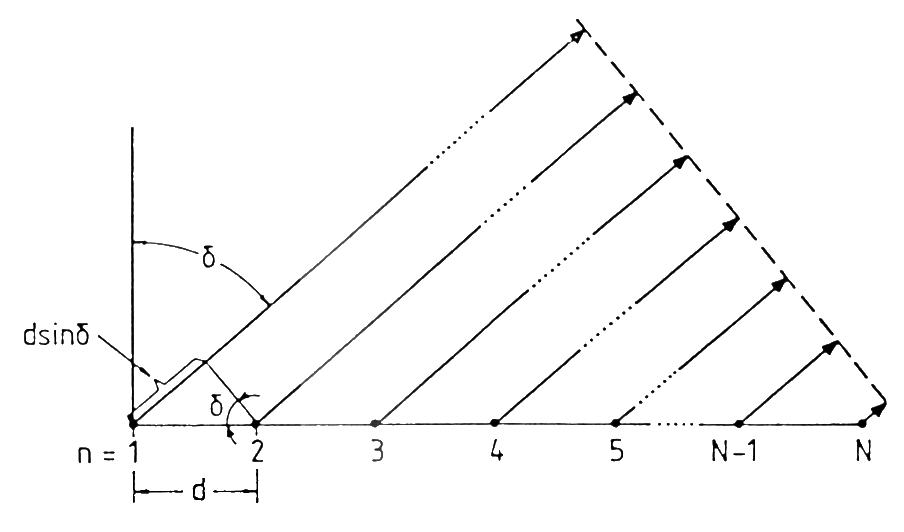
\includegraphics[width=0.7\textwidth]{images/PAradiationPattern}
	\caption{Wave vectors radiated from isotropic antenna elements with spacing d under zenith angle $\delta$ \citep[c.f.][Figure 10]{roettger1989instrumental}}
	\label{fig:radiationPattern}
\end{figure}

Combining the different distances to the targets with the appropriate current for each array element and inserting it into equation \ref{eq:iso_radiator} leads to the radiation pattern for each antenna, denoted in eq. \ref{eq:fieldsOfArray}. 

%\begin{equation}
\begin{eqnarray}
	E_1(\delta) &=& I_0 \frac{e^{-jkr}}{4\pi r}\\
        &\vdots& \\
	E_N(\delta) &=& I_0 e^{j\varphi_{N}} \frac{e^{-jk[r - (N-1)d\sin\delta]}}{4\pi r}
	\label{eq:fieldsOfArray}
\end{eqnarray}
%\end{equation}

Assuming that all array element antennas are the same and have the same pattern, the fields can be summed using the superposition principle, to obtain the Array Pattern. Thus using equation \ref{eq:iso_radiator} we can obtain


\begin{eqnarray}
	E_\delta &=& E_1(\delta) + \dots + E_N(\delta) \\
	 &=& E_0 [1 + e^{j\varphi_2 + k d \sin \delta} + \dots + e^{j[\varphi_N + (N-1) k d \sin \delta]}]
\end{eqnarray}

By assuming that the Array Element Pattern $E_0$ for each elements is constant, the Array Pattern will only be affected by the Array Factor. Thus, by applying the substitution $\gamma = \varphi + kd\sin\delta$ we can rewrite the Array Factor as follows:
\begin{equation}
	AF = \sum_{n=1}^N e^{j(n-1)\gamma}
\end{equation}
Multiplying both sides with $e^{j\gamma}$, we can get rid off of the subtraction on the right side, and by subtracting the Array Factor from both sides, we can free the equation from the sum on the right side, which gives us the following expression for the Array Factor:
\begin{equation}
	AF = \frac{e^{jN\gamma} - 1}{e^{j\gamma} - 1} = e^{0.5j(N-1)\gamma} \frac{\sin(\frac{N\gamma}{2} )}{\sin(\frac{\gamma}{2} )}
\end{equation}

If we now shift the position of the array, so that the center of the is located at $N = 1$ (which represents a shift by $-\varphi$), the complex exponential expression reduces to 1. Inserting the re-substitution and expressing the wavenumber with $k = \frac{2\pi}{\lambda}$, we get the following real expression for the Array Factor:
\begin{equation}
	AF = \frac{\sin(\frac{Nd\pi\sin\delta}{\lambda})}{\sin(\frac{d\pi\sin\delta}{\lambda})}
	\label{eq:AF}
\end{equation}

%%%%%%%%%%%%%%%%% TASK 1 %%%
\section{Optimal distance between array elements}
Using the derived Array Factor equation in chap. \ref{chap:derivation}, the Array Pattern can be plotted using Matlab (). The Array Factor was normalized to the number of Array Elements, to be able to compare the results in an easier way.

\begin{figure}[h!]
	\centering
	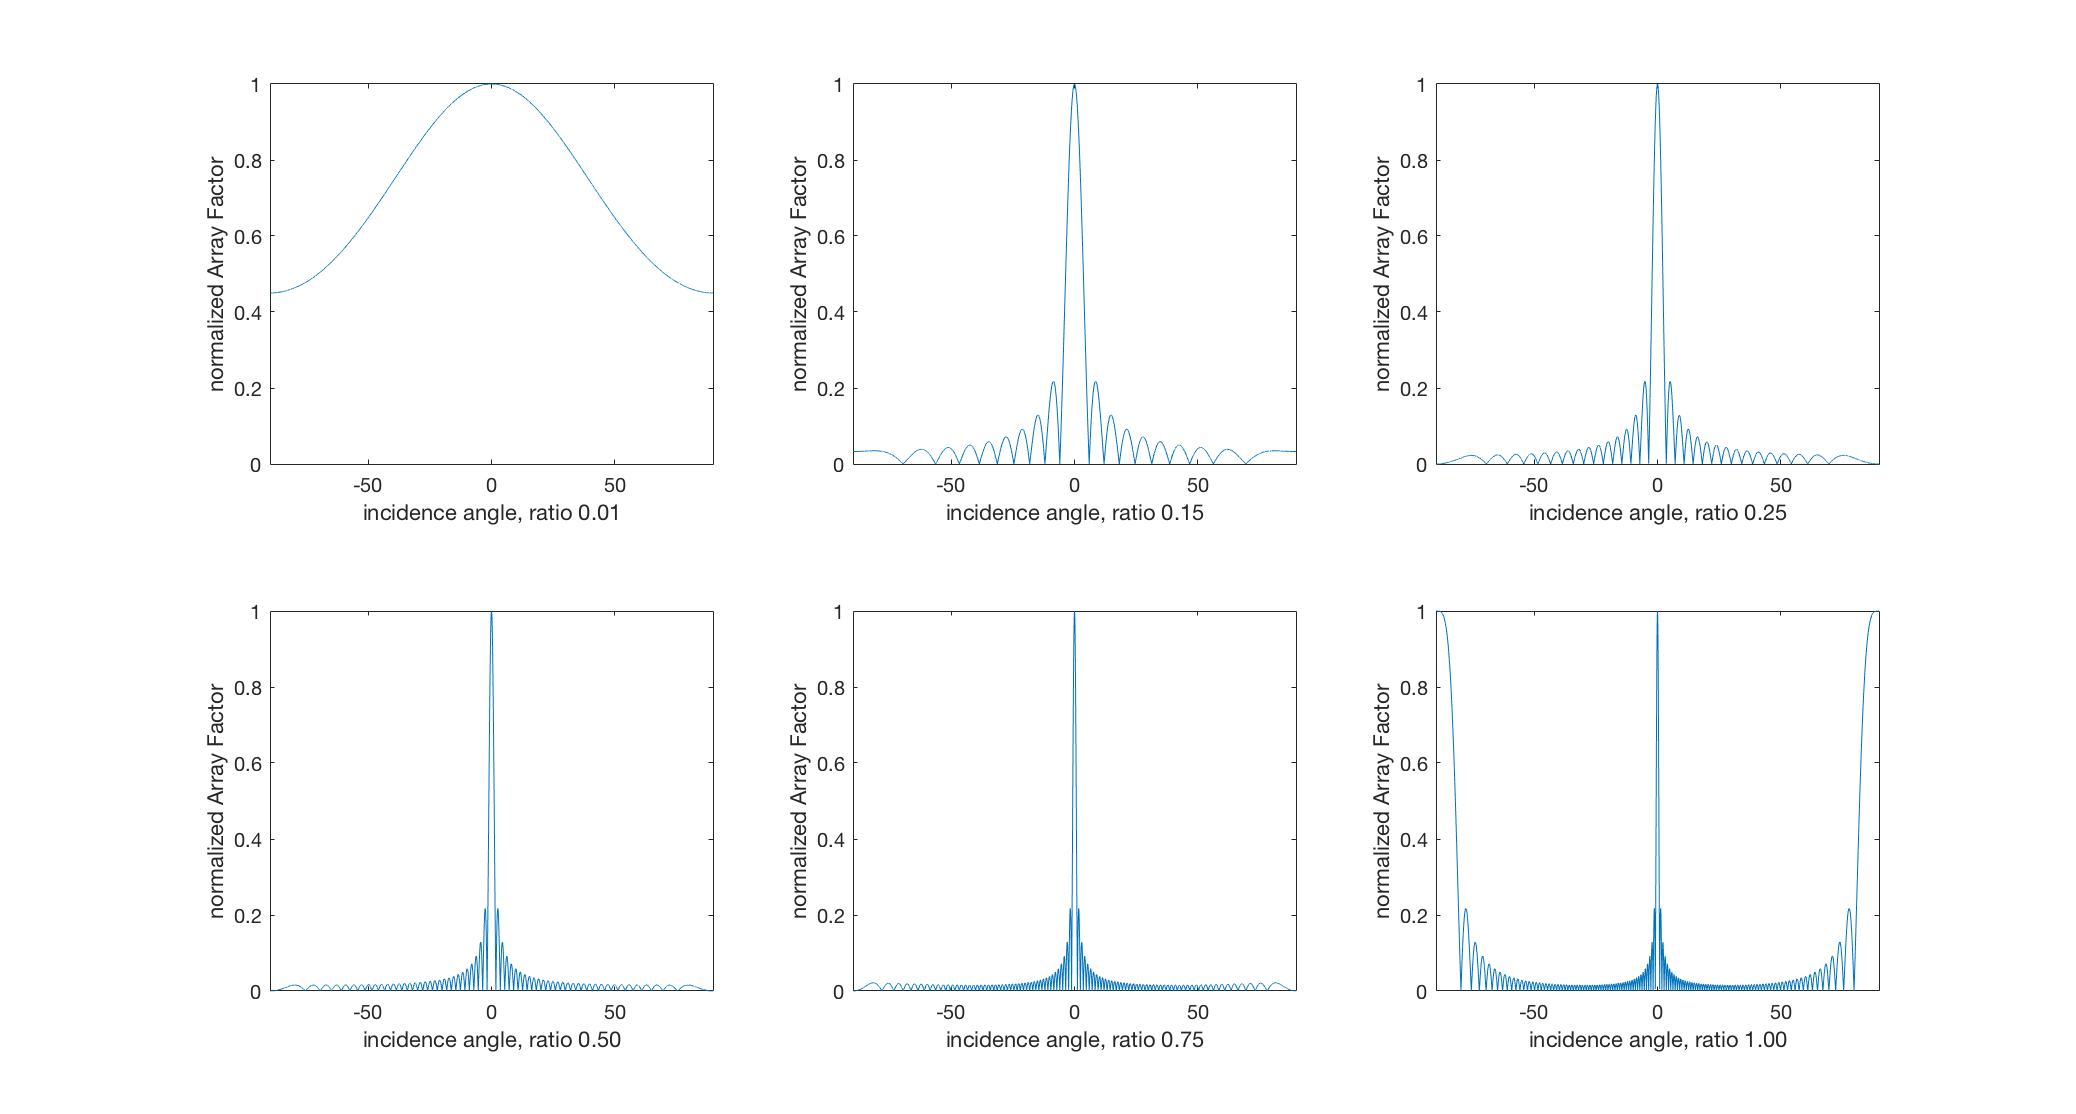
\includegraphics[width=\textwidth]{images/distanceVariation}
	\caption{Array Pattern with various distance-to-wavelength ratios}
	\label{fig:distance}
\end{figure} 

According to Richards et. al. \citep{richards2010principles}, the maximum allowable distance between the array elements must fulfil the equation
\begin{equation}
	\Delta x \leq \frac{\lambda}{(1 + |\sin\theta_S |)}
	\label{eq:deltaX}
\end{equation}

with $\theta_S $ being the desired maximum scan angle of the phased array. Inserting the appropriate values for the given antenna parameters leads to a ideal spacing of 2.8826m, which corresponds to an ideal distance-to-wavelength ratio of 0.5. The maximum spacing between two adjacent antennas is seen as ideal, since this minimizes the cost of the antenna setup and electronics \citep{richards2010principles}, but is still small enough so that grating lobes are pushed outside the scan window.

%%%%%%%%%%%%%%%%% TASK 2 %%%
\section{Number of antenna elements}
Using again the Array Factor equation \ref{eq:AF}, the number of array Elements is varied and the resulting (normalized) Array Factor is plotted against the scanning angle. For these plots the distance-to-wavelength was set to 0.5, according to the results from the previous chapter. As one can see in fig. \ref{fig:varyingElements}, the main lobe gets "sharper" and thinner, the more Array Elements are used. But we also get more sidelobes the more Array Elements we have.

\begin{figure}[h!]
	\centering
	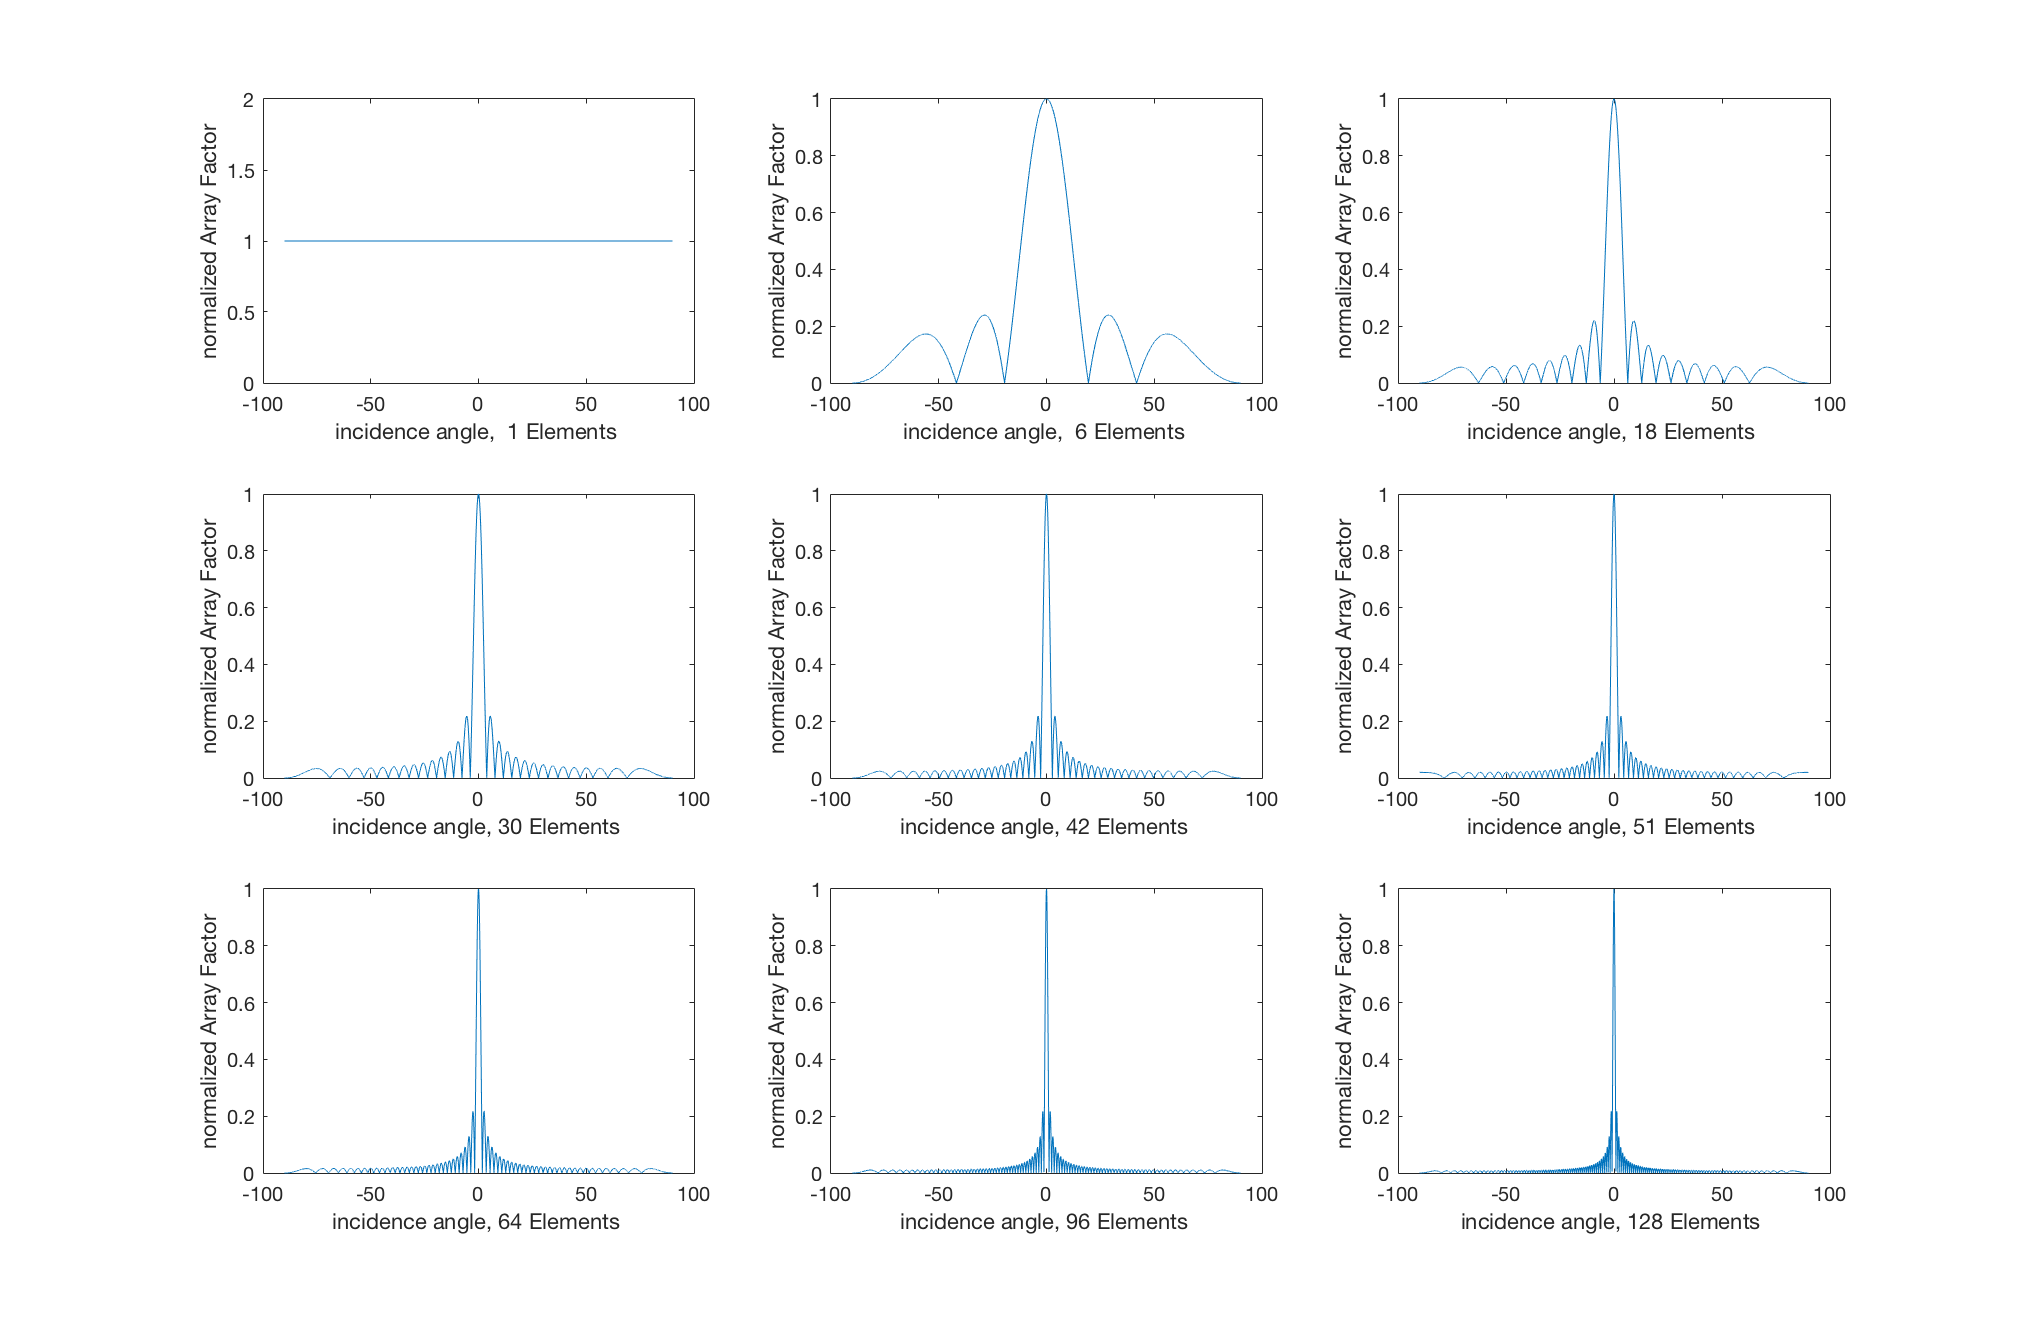
\includegraphics[width=\textwidth]{images/elementVariation}
	\caption{varying amount of array elements, with fixed $\frac{d}{\lambda}$-ratio of 0.5}
	\label{fig:varyingElements}
\end{figure}



%%%%%%%%%%%%%%%%% TASK 3 %%%
\section{Spatial Weighting}
To further suppress the side lobes, one can apply a technique called "spatial weighting". Here, the distance between the elements is increased, starting from the middle of the antenna.\todo{language}
Since now the distance between the Array Elements are not uniform, and thus the phase shift in-between is neither, we can not use the simplified equation \ref{eq:AF}, derived in chapter \ref{chap:derivation}, but must use the initially given expression in \ref{eq:orig} \citep{roettger1989instrumental}.

\begin{figure}[h!]
	\centering
	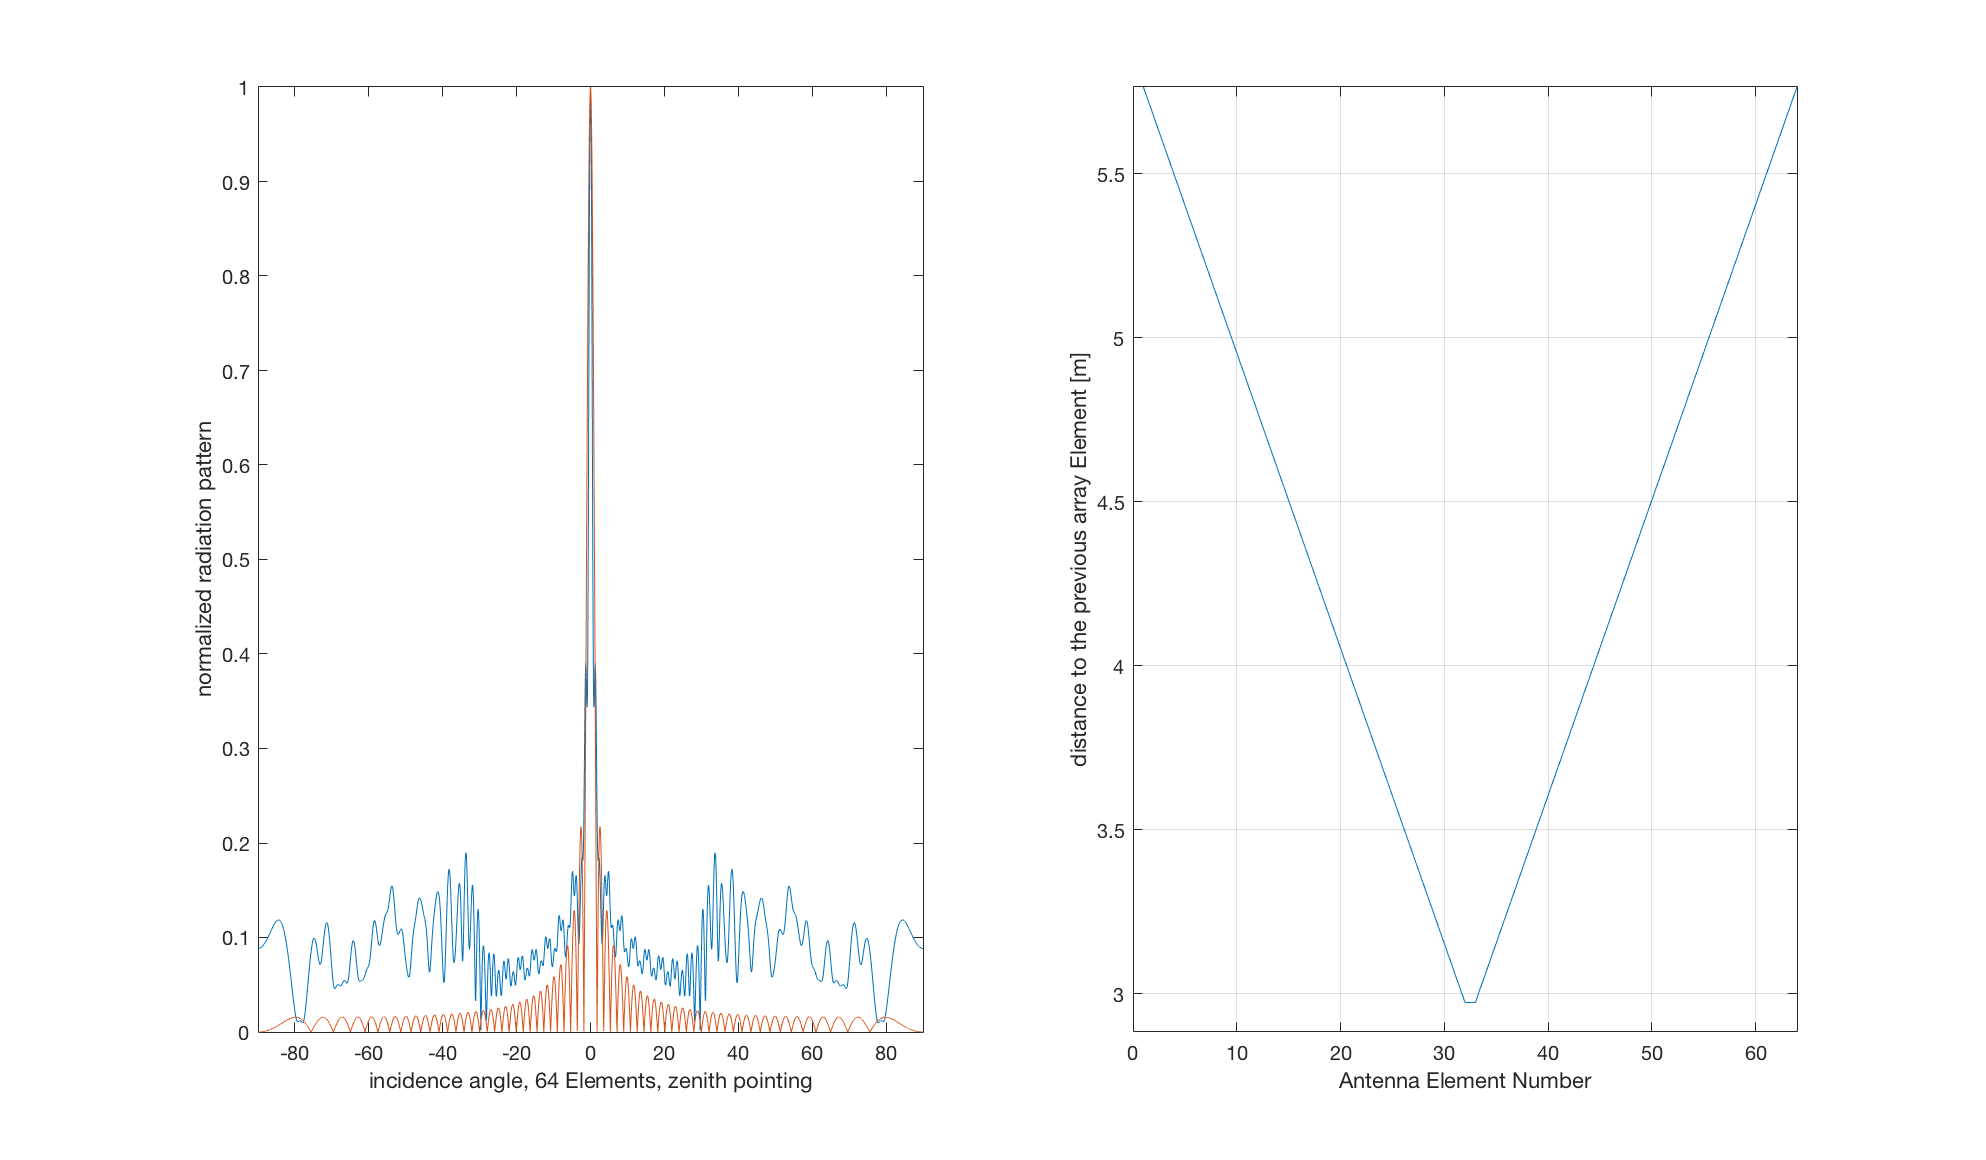
\includegraphics[width=\textwidth]{images/triangularSpatialWeight}
	\caption{Spatial Weighting for Array Elements}
	\label{fig:triangWeight}
\end{figure}

Comparing fig. \ref{fig:triangWeight} with fig. \ref{fig:varyingElements} (64 Elements), we can see, that the sidelobes right next to the main lobe are heavily suppressed when a triangular weighting function is used, to increase the distance in the outer elements. However, this introduces an increase of sidelobe amplitudes in higher incidence angles, which might not be desired in all applications.



%%%%%%%%%%%%%%%%% TASK 4 %%%
\section{Optimal Design for antenna array}


%%%%%%%%%%%%%%%%% TASK 5 %%%
\section{Main lobe maximum and width}


%%%%%%%%%%%%%%%%% TASK 6 %%%
\section{Radiation pattern change when non-vertical beam}


%%%%%%%%%%%%%%%%% TASK 7 %%%
\section{Electrical Weighting}
